%

%
%
%
%
%


%
%

%


%

%

%

%

%

%

%

%

%
%

%
%


%



%
%
%
%
%
%
%
%
%
%
%
%
%
%
%
%
%
%
%




%
%

\begin{figure*}[t]
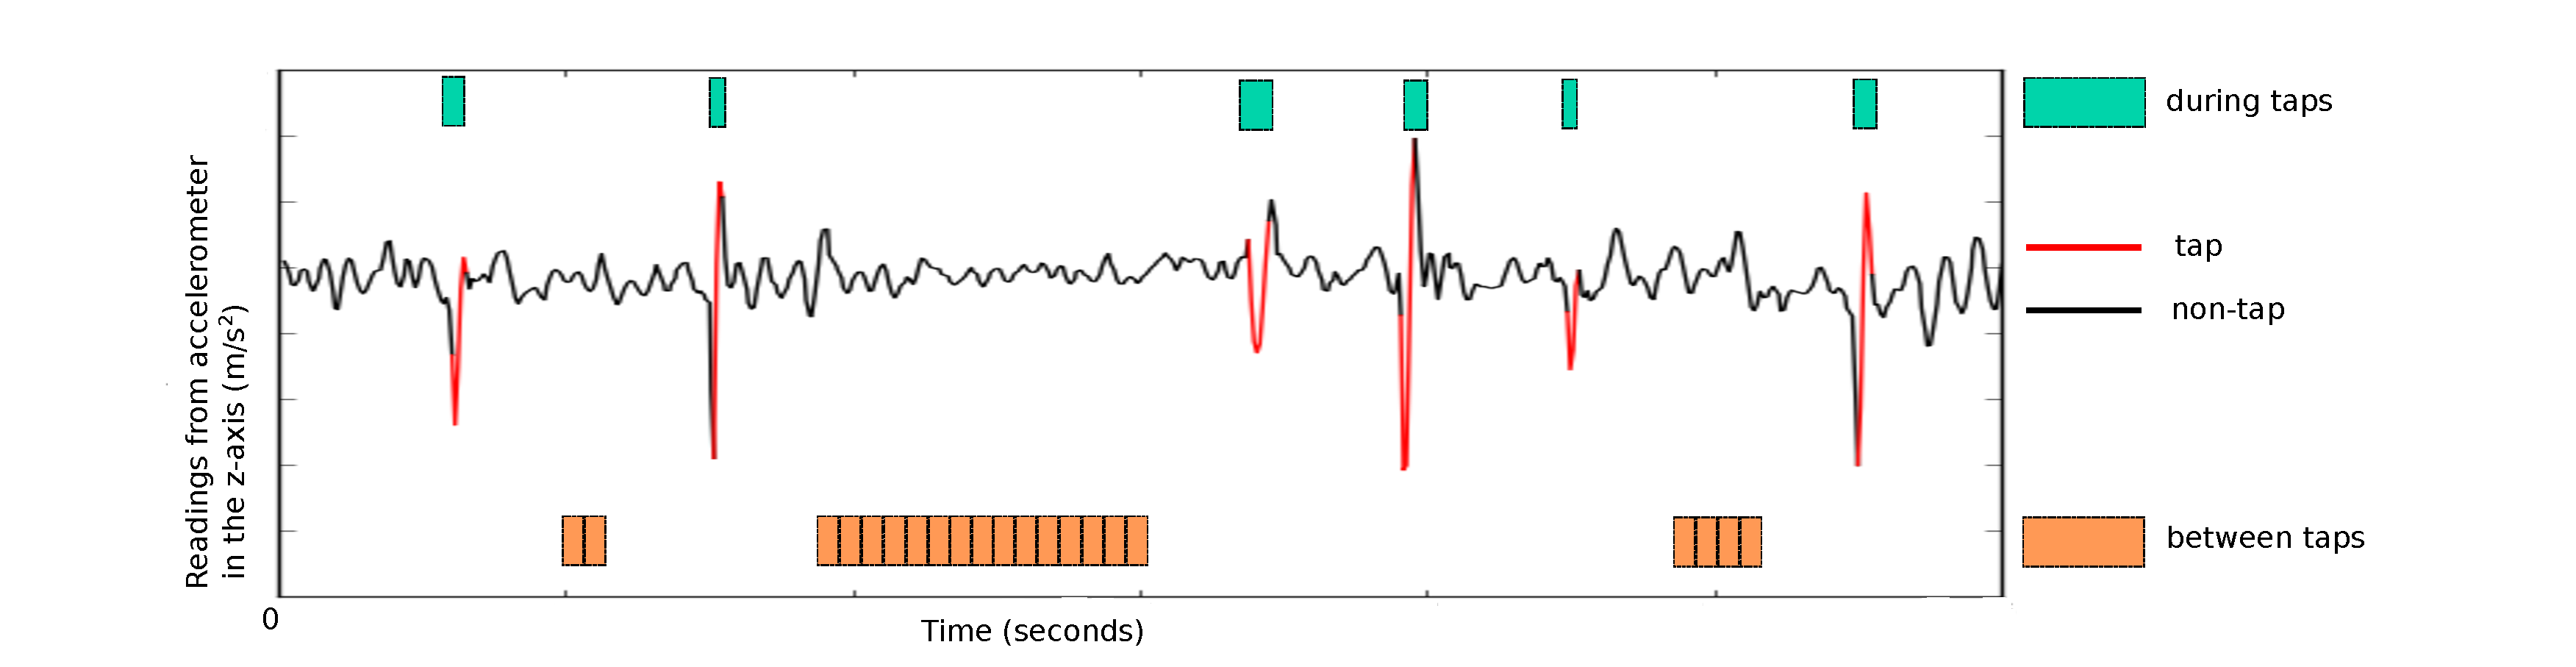
\includegraphics[width=1\linewidth]{plots/betweenExplainedFinal.pdf}
%
%
%
%
\caption[]{HMOG features extracted {\em during} and {\em between} taps. The figure shows a sample of readings from the z-axis of accelerometer in sitting condition.}
\label{fig:betweenExplained}
\end{figure*}








\subsection{Why HMOG Features Perform Better During Walking}

\begin{figure}[t]
%
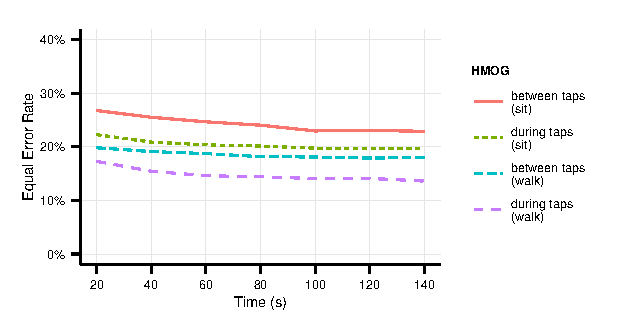
\includegraphics[width=1.1\linewidth]{plots_R/auth_between_taps.pdf}
\caption[]{Performance of HMOG features extracted {\em during}  and {\em between} taps. $X$-axis shows authentication time in seconds.}
\label{fig:betweenTapsSM}
%
%
%
%
%
%
\end{figure}

%

%

%

 %

%


%

We investigated why HMOG features performed better during walking. Specifically, we investigated whether the high authentication accuracies of HMOG features during walking were due to hand movements caused by taps, or due to movements caused by walking, or a combination of both. %

\paragraph{Experiment setup} We extracted 64 HMOG features from two segments of an accelerometer/gyroscope signal: (1) {\em during tap}, as discussed in previous sections; and (2) {\em between taps}, in which HMOG features were extracted when the user was \textit{not} tapping the screen (see Figure~\ref{fig:betweenExplained}). In (2), the signal between taps was segmented into non-overlapping blocks of 91~ms; one HMOG feature vector was extracted from each block. 
We selected 91ms as the block size because it was the median duration of a tap in our training data. This ensured that the number of sensor readings used to extract a HMOG feature vector {\em between} and {\em during} tap remained same. %

%

HMOG features extracted {\em during} taps use sensor readings from 100~ms before and 200~ms after a tap event (see Section \ref{sectionFeatures}). We extracted HMOG features {\em between} taps starting 300~ms after a tap until 300~ms before the next tap, to avoid any overlap between {\em during} and {\em between} HMOG features.%
%
%
%
%
%
 



%

%


%

%
%
%
%
%


%

%

%

%



%
%
The average number of the training vectors per user for HMOG {\em during} taps was 1122 for sitting, and 1186 for walking. For {\em between} taps, it was 7692 for sitting and 7462 for walking. %
The average number of testing vectors per user for HMOG features {\em during} taps was 897 for sitting and 972 for walking. For  {\em between} taps, it was 5885 for sitting and 5768 for walking. Verification experiments were performed using SM. 

%
%
%

%

\paragraph{Performance of HMOG Features Extracted During vs. Between Taps}  
We compared HMOG features extracted during taps with the same features extracted between taps for sitting and walking conditions. For sitting, HMOG features extracted {\em during} taps performed consistently better  than those extracted {\em between} taps (see EERs in Figure~\ref{fig:betweenTapsSM}). This indicates that HMOG features were able to capture distinctive hand micro-movement patterns when the users tapped on the phone. %
%
%
Similarly, for walking, HMOG features extracted {\em during} taps performed better than those extracted {\em between} taps (see EERs in Figure~\ref{fig:betweenTapsSM}). This again indicates that HMOG features capture user's distinctive hand micro-movement patterns when the user is tapping, regardless of the motion condition.
%


%
%

\paragraph{Impact of Walking on HMOG Features Extracted Between Taps} HMOG features extracted  {\em between} taps during walking outperformed the same when extracted during sitting (see {\em between} tap EERs for sitting and walking in Figure~\ref{fig:betweenTapsSM}). This indicates that HMOG features capture distinctive movements induced by walking, even in the {\em absence} of tap activity.%
%
%


\bigskip
Supported by the above results, the high authentication accuracies achieved by HMOG features during walking can be jointly attributed to: (a) the distinctiveness in hand movements caused by tap activity and (b) the distinctiveness in movements caused by walking. %


%

%
%

%

%
%
%

%

%
%

%

%


%

%


%
  
%


%


%

%

%



%





%

%

 %



%

%




%

%
%
%
%
%
%
%
%
%
%
%
%
%
%

%
%
%
%
%
%
%
%
%
%
%
%
%
%


%

%

%
%
%
%
%



%

%

%
%
%
%
%

